\documentclass{article}
\renewcommand\refname{Bibliografie}
\usepackage{blindtext}
\usepackage{amsmath,amssymb}
\usepackage{graphicx}
\usepackage[]{algorithm2e}
\title{The Boyz - Raport Tehnic}
\date{Aprilie, 2020}
\author{ Blaj Marius, Lipan Radu Matei, Anul 3, A1}
\begin{document}
\maketitle

"The Boyz" este aplicatia propusa de noi pentru cursul de "Cloud Computing" din anul 3, semestrul 2. Aceasta are ca si scop ajutarea utilizatorului in a-si gasi noi coechipieri cu care sa joace jocuri online sau chiar "antrenori" pentru aceste jocuri. In cadrul aplicatiei poti plati persoane necunoscute sa joace un joc video cu tine de un anumit numar de ori, cu scopul de a cunoaste oameni noi cu aceleasi interese ca tine sau chiar pentru a deveni mai bun in jocul respectiv in cazul in care angajezi un "antrenor".

Desi, la prima vedere, ideea acestei aplicatii nu pare foarte atractiva, aceasta poate avea un succes rasunator in contextul. In ultimii ani industria jocurilor a devenit foarte puternica, jocuri precum "GTA V" devenind unul dintre cele mai profitabile produse de entertainment din toate timpurile (6 miliarde de dolari in venituri) depasind filme precum "Avatar", "Star Wars" si "Gone With The Wind"\cite{gameindustry}. Totodata achizitiile din ultimi ani a diferitelor platforme dedicate streamingului de jocuri video precum achizitia twitch-ului de catre Amazon sau a mixer-ului de catre Microsoft semnalizeaza o posibila dezvoltare si mai puternica a acestui spatiu.

\section{Aplicatii similare}
\subsection{E-pal}
Epal.gg\cite{epal}(cunoscut anterior ca egirl.gg) este momentan cel mai cunoscut astfel de site. Lansat in Februarie 2020 acesta a cunoscut o crestere foarte rapida si puternica intr-un timp foarte scurt datorita interfetei complete si intuitive si a versatilitatii serviciilor oferite(diferite jocuri, preturi, timezone-uri, servere din care utilizatorii pot alege).

Dupa cum se poate observa si din a doua statistica din Figura \ref{fig:epal-stat-1}, majoritatea utilizatorilor vin direct pe site, si nu prin intermediul unei cautari. Acest lucru se datoreaza ingenioasei strategii de marketing focusate in special catre Twitch si Youtube Gaming. Astfel au avut deschidere la numerosi posibili consumatori si s-au facut cunoscuti in aceste comunitati foarte rapid. Un dezavantaj a fost faptul ca nu erau pregatiti pentru un raspuns pozitiv atat de puternic si in prima luna site-ul a picat de nenumarate ori de fiecare data cand un streamer sau youtuber mai mare facea publicitate aplicatiei.
\begin{figure}[ht]
\centering
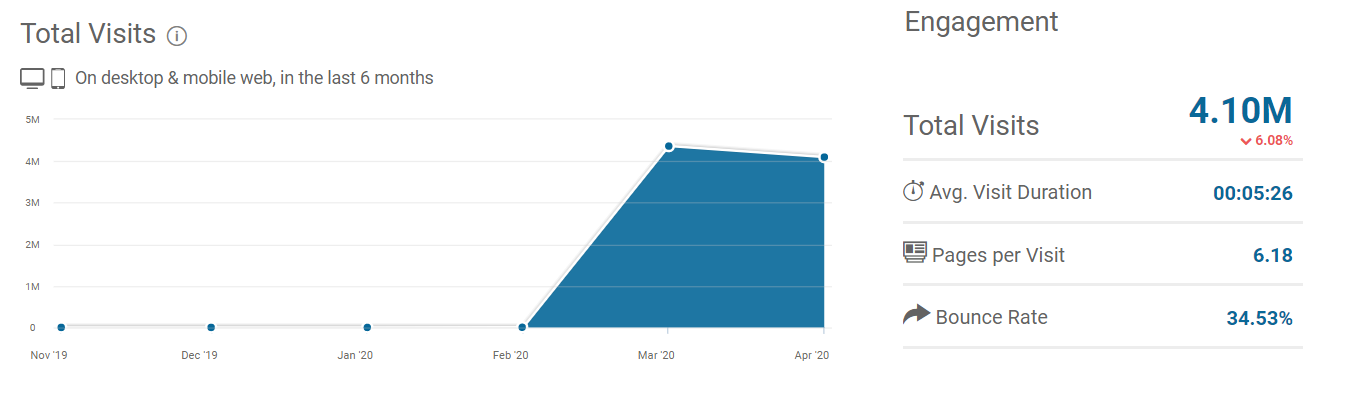
\includegraphics[width=0.95\textwidth]{img/epal-stat-1.png}
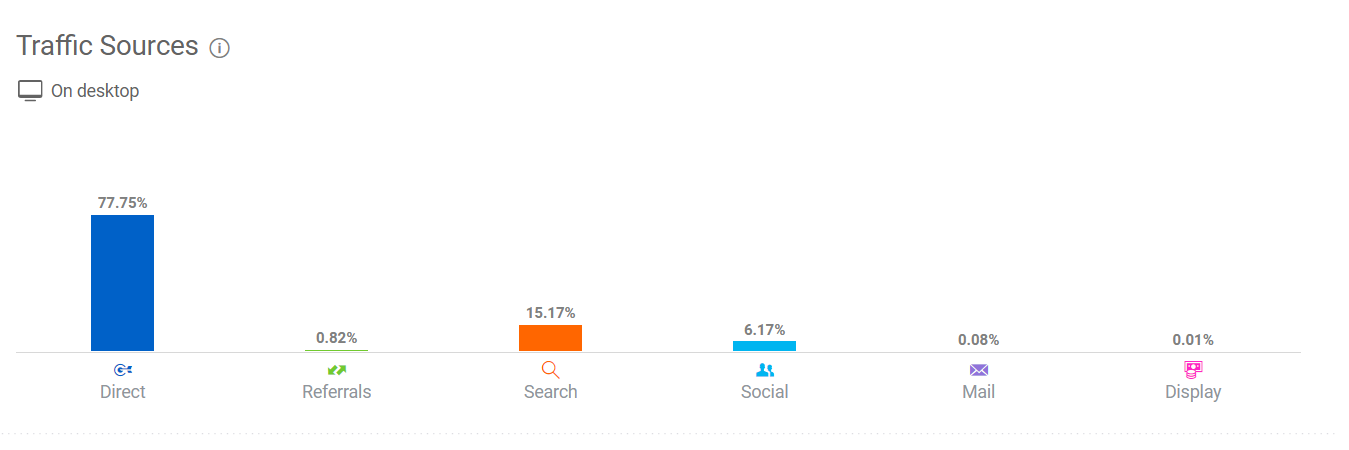
\includegraphics[width=0.95\textwidth]{img/epal-stat-2.png}
\caption{Traficul site-ului epal.gg de la lansare pana azi\cite{epalstats}} 
\label{fig:epal-stat-1}
\end{figure}

\subsection{Gamer Sensei}
GamerSensei\cite{gamersensei} este un alt astfel de site care spre deosebire de Epal se axeaza doar pe angajarea de jucatori profesionisti in scopul antrenarii altor jucatori. Aceasta aplicatie este destinata mai mult spatiului de Esports, puternic dezvoltat in ultimii 5 ani. Utilizatorii sunt adesea echipe care vor sa se lanseze pe scena lor de esports si care cauta sa fie pusi in contatct cu fosti jucatori profesionisti pentru a putea concura si pentru a avea o sansa in a se face renumiti in domeniul lor.
\section{Business Canvas}

In Figura \ref{fig:canvas} putem observa Business Canvas-ul pentru aplicatia noastra. Aceasta va fi construita peste serviciile de cloud de la Google pentru a putea face fata la variatiile mari de trafic aduse de o strategie de marketing asemanatoare celei puse in practica de Epal. Am ales Google deaorece este mult mai usor de folosit decat competitorii, salvand astfel timp de dezvoltare, in timp ce preturile sunt foarte asemanatoare cu cele oferite de catre acestia.

Principalul flux de venituri ar fi o taxa de aproximativ 5\% luata de catre aplicatie din toate achizitiile facute in cadrul acesteia. Paypal si Stripe ofera posibilitatea procesarii sigure de tranzactii dar si adaugarea unei astfel de taxe automate platilor facute prin intermediul conturilor de tip business. 

Principalele costuri si activitati ar fi legate doar de dezvoltarea aplicatiei, stocarea acesteia pe serviciile de cloud dar si marketingul ei online prin reclame sau prin intermediul twitch streamerilor sau a youtuberilor. Relatia cu consumatorul nu este una foarte puternica momentan, acesta doar realizand achizitia prin intermediul site-ului. Dupa realizarea cu succes a acesteia nu mai are nevoie de produsul oferit de noi.

\begin{figure}[ht]
\centering
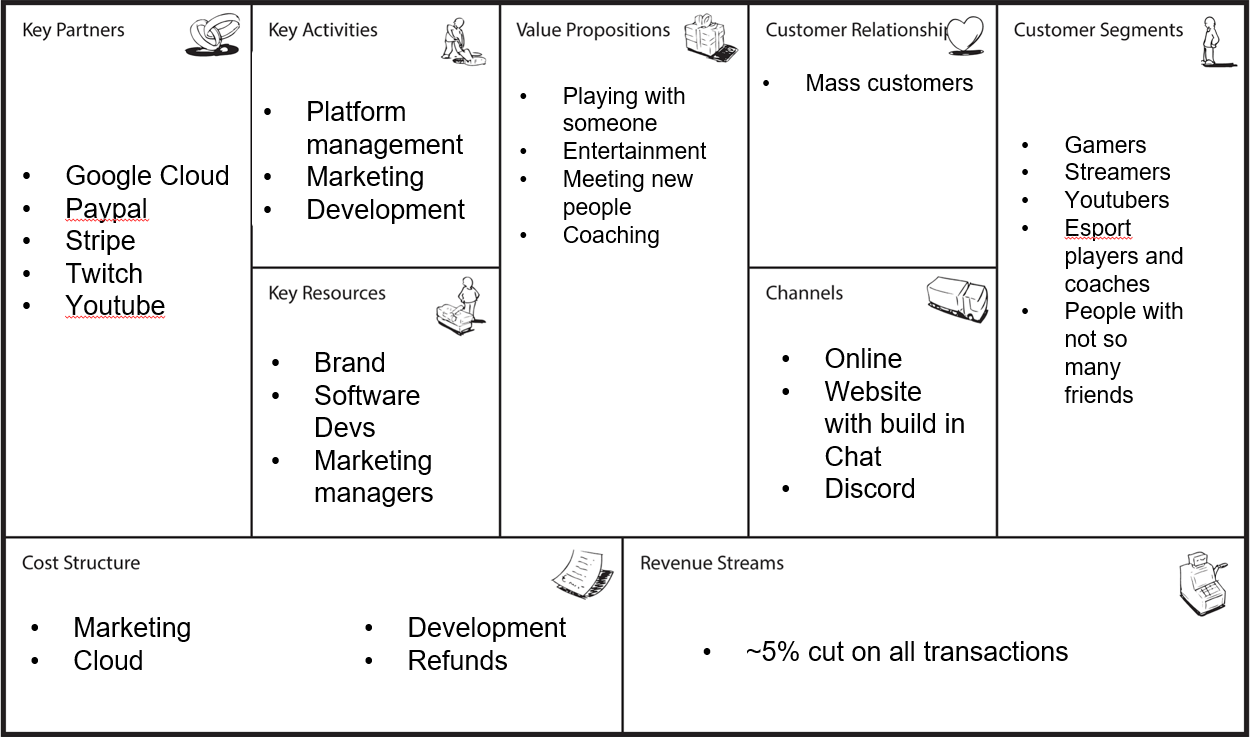
\includegraphics[width=1\textwidth]{img/canvas.png}
\caption{Business Canvas pentru The Boyz} 
\label{fig:canvas}
\end{figure}

\section{Arhitectura}

In Figura \ref{fig:architecture} poate fi observata arhitectura aplicatiei la momentul actual. Am recurs la o abordare serverless, fiecare functie oferind un numar mic de endpoint-uri strans legate intre ele(\textbackslash users, \textbackslash orders, de exemplu). Aceasta abordare permite scalarea doar a zonelor puternic folosite de aplicatie la momentul actual. De exemplu: un streamer tocmai face reclama site-ului si un numar foarte mare de utilizatori intra pe site. Dintre acestia, foarte putini vor dori sa utilizeze site-ul la momentul actual si pentru a plasa comenzi sau pentru a vorbi utilizand chat-ul inclus. Astfel, folosind arhitectura bazata pe functii, functia care se ocupa de \textbackslash users va fi scalata puternic iar celelalte functii care ofera \textbackslash orders sau \textbackslash messages nu vor fi scalate aproape deloc in loc ca instante pentru tot back-end sa fie initializate odata cu cresterea traficului.

Toate celelalte servicii folosite de aplicatie sunt vizibile si in schema arhitecturala. Avem astfel: Firebase authentication pentru logarea utilizatorilor, Realtime Database pentru a salva datele necesare aplicatiei, Cloud Storage pentru a salva pozele de profil, inregistrarile audio, etc și Cloud Speech To Text Service pentru a obtine o descriere a utilizatorului din inregistrarea oferita de acesta la crearea contului. 

Totodata, ne-am folosit si de trigger-urile puse la dispozitie de Firebase Realtime Database pentru a asculta anumite modificari din interiorul bazei de date pentru a porni functiile cloud necesare dezvoltarii unui modul de chat in timp real.

\begin{figure}[ht]
\centering
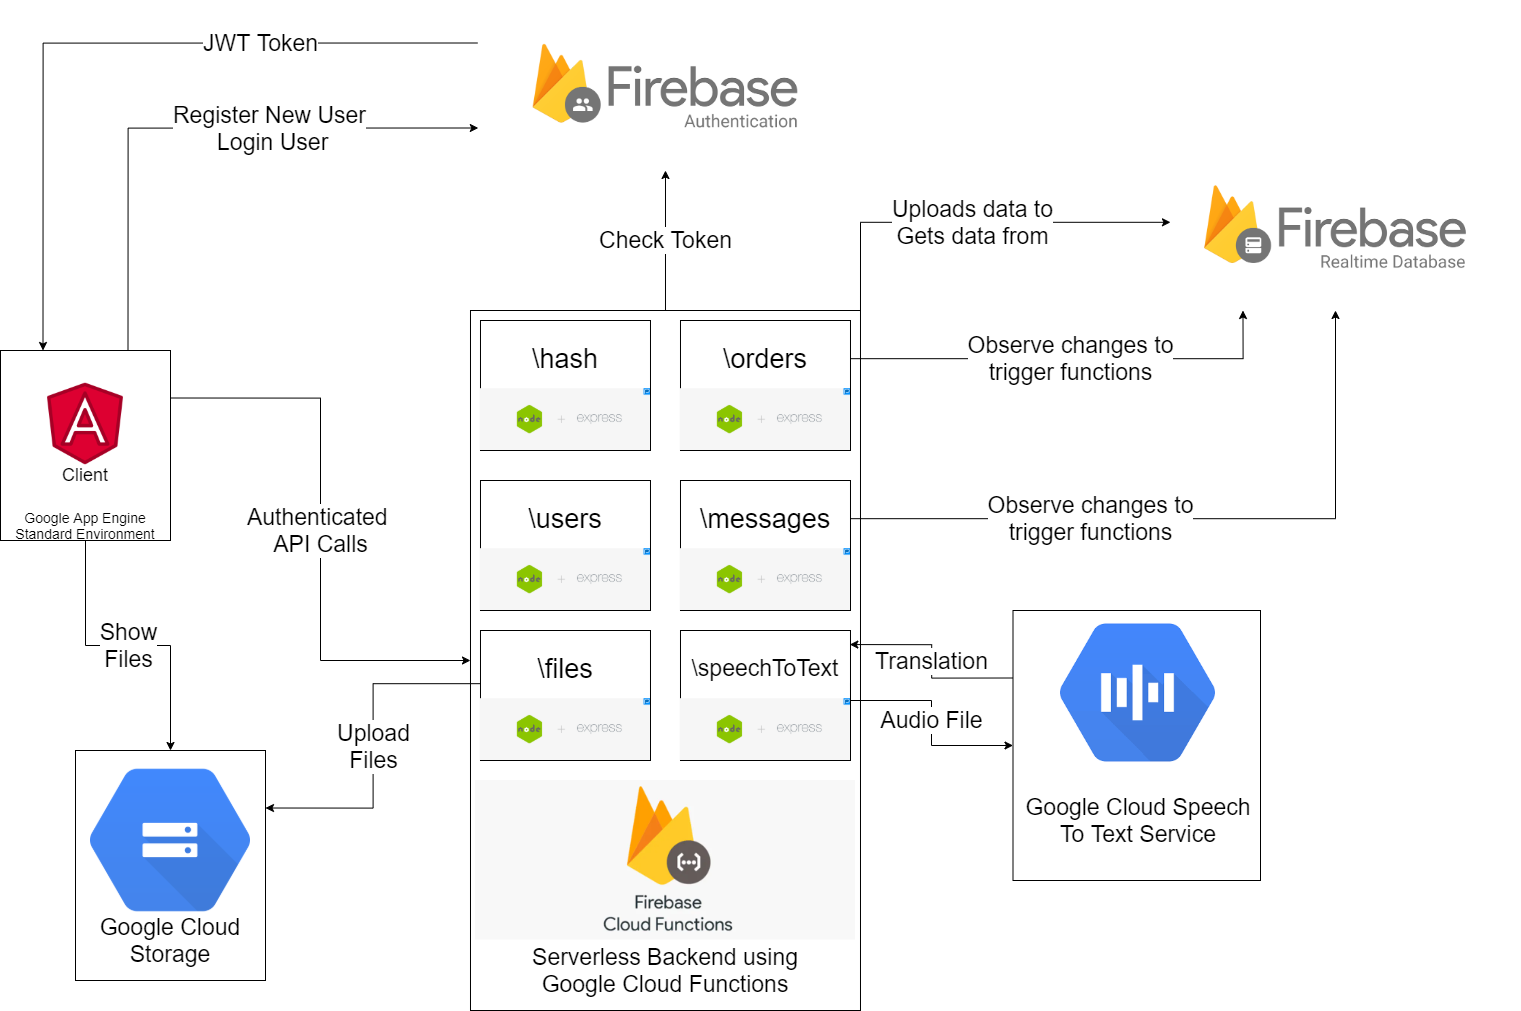
\includegraphics[width=1\textwidth]{img/CC_architecture.png}
\caption{Arhitectura actuala a aplicatiei The Boyz} 
\label{fig:architecture}
\end{figure}

\section{Diagrame Use-Case}

\begin{figure}[ht]
\centering
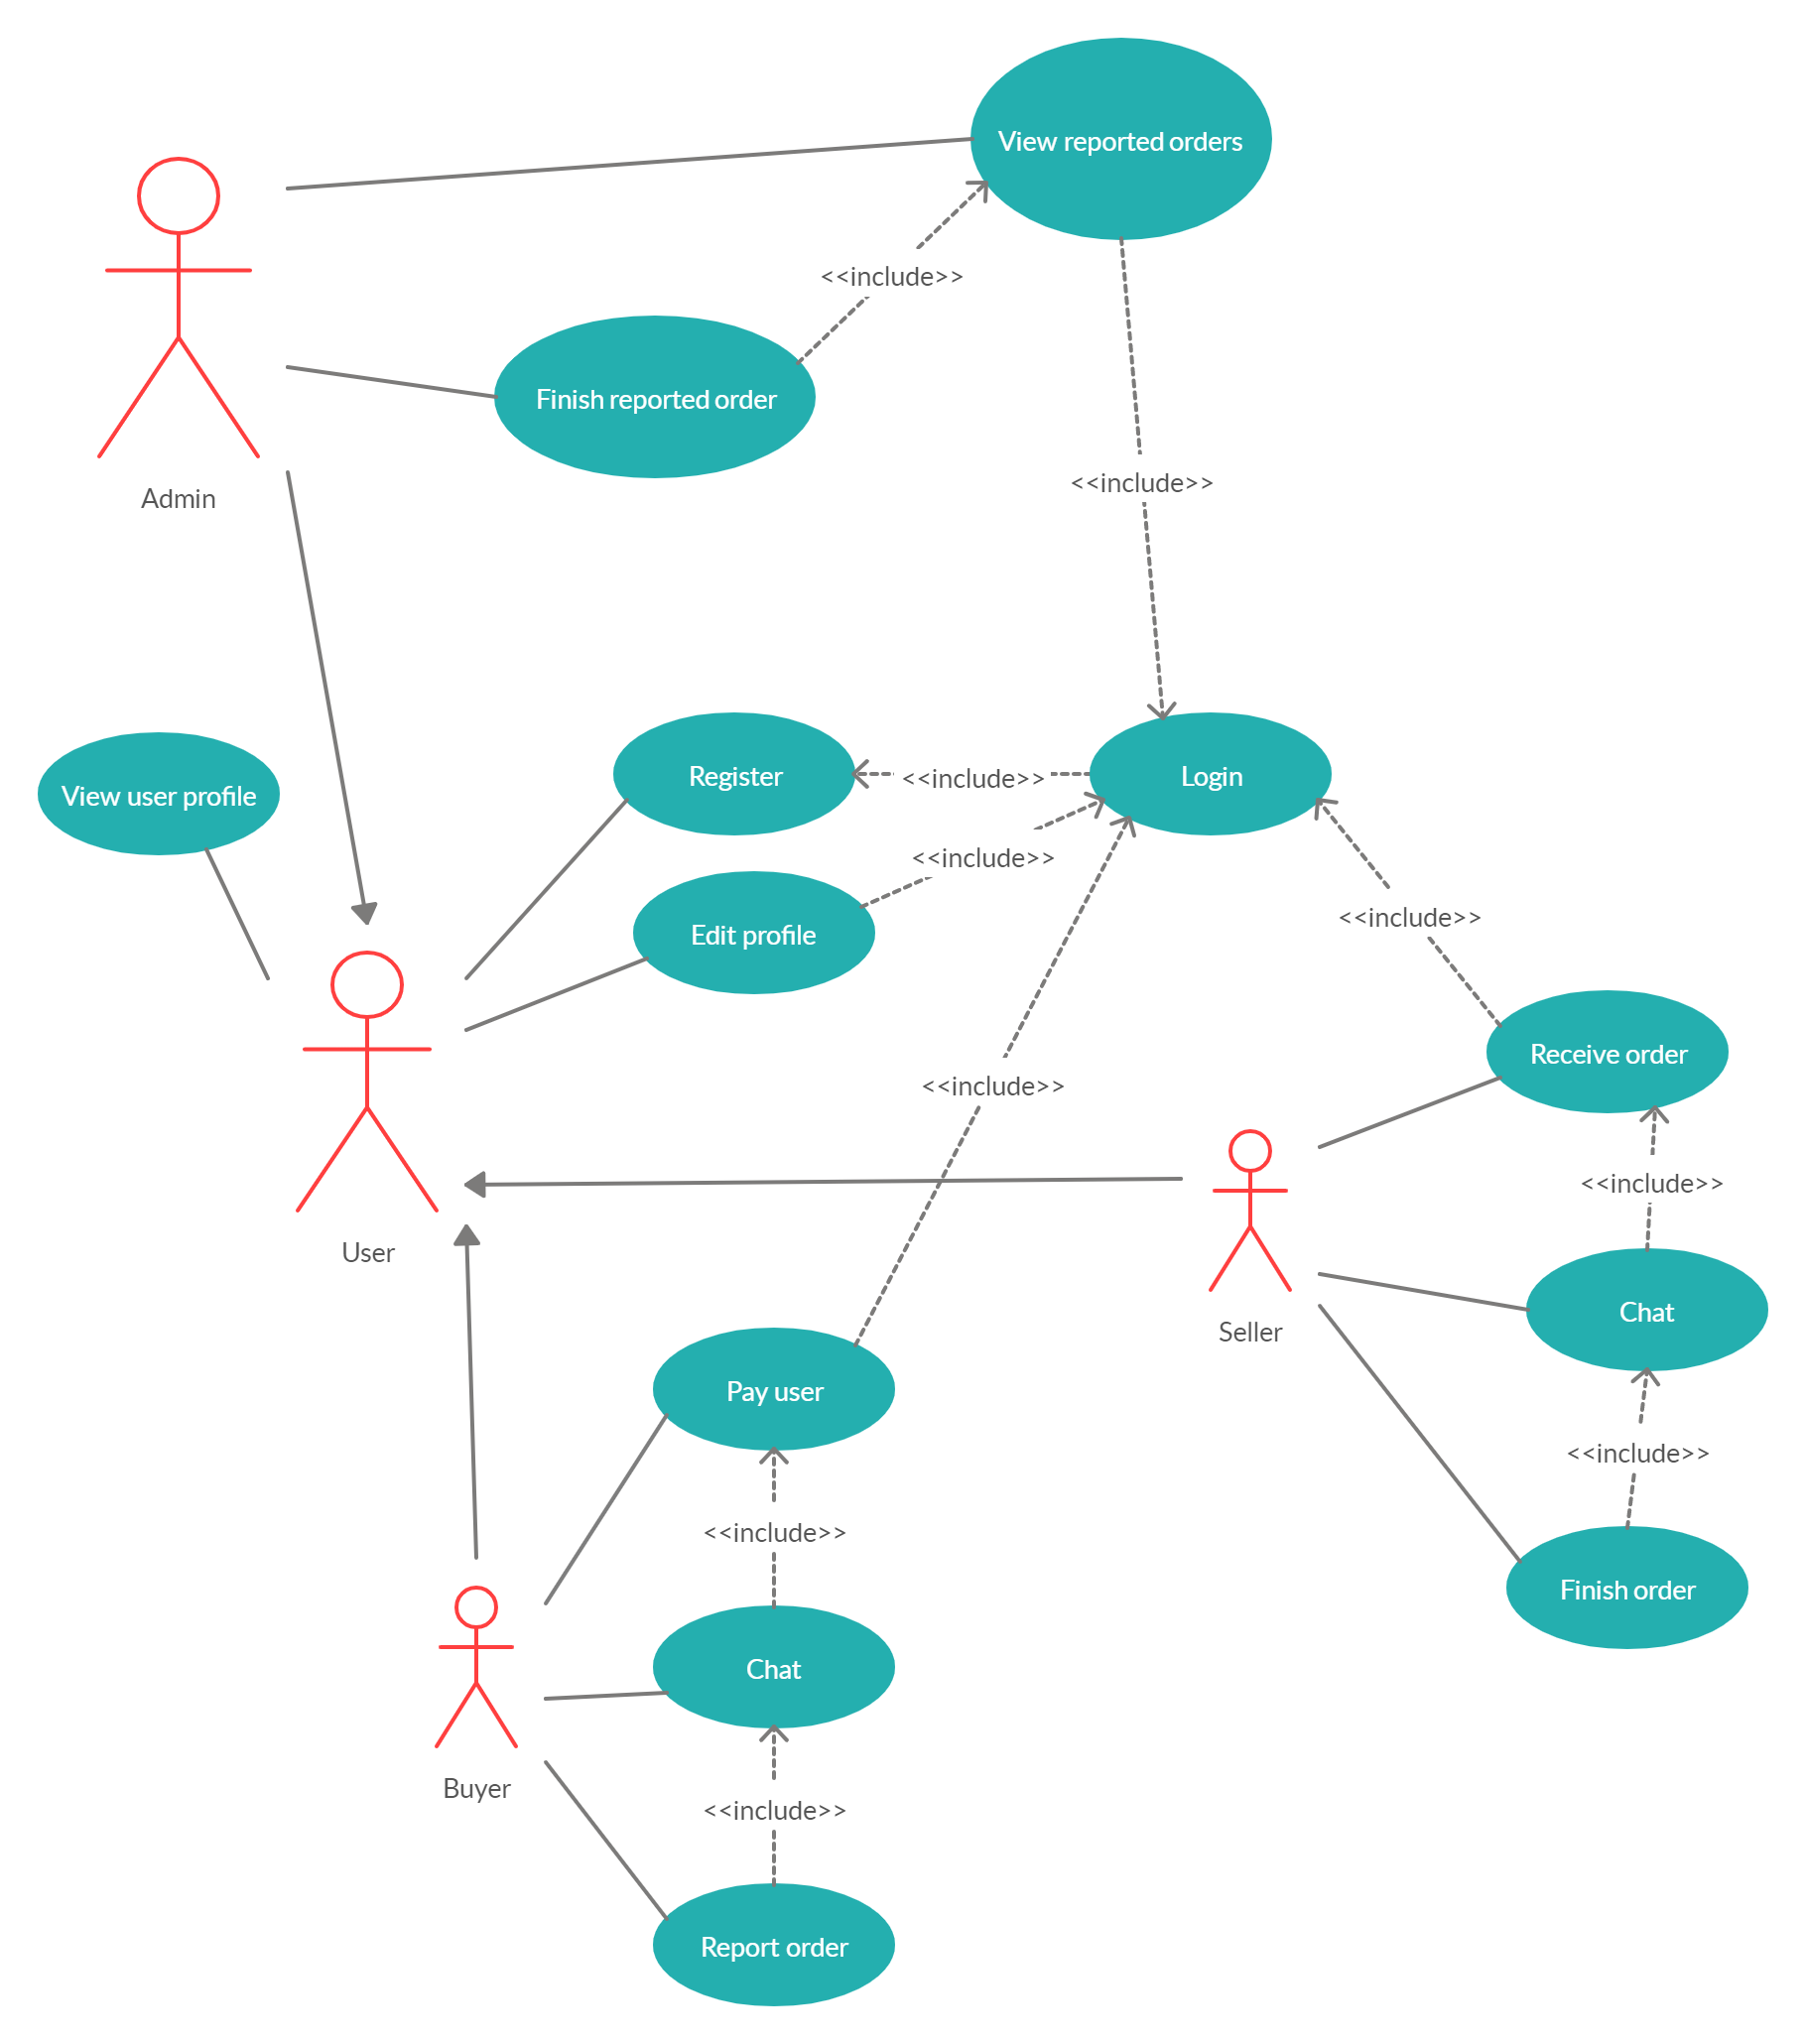
\includegraphics[width=1\textwidth]{img/use-case.png}
\caption{Arhitectura actuala a aplicatiei The Boyz} 
\label{fig:architecture}
\end{figure}

\begin{thebibliography}{9}

\bibitem{epal}
E-pal: principala sursa de inspiratie pentru acest proiect,
\\\texttt{https://www.epal.gg}

\bibitem{gamersensei}
GamerSensei: aplicatie similara care se focuseaza mai mult pe antrenori,
\\\texttt{https://www.gamersensei.com/}

\bibitem{gameindustry}
James Batchelor for gameindustry.biz: GTA V is the most profitable entertainment product of all time,
\\\texttt{https://www.gamesindustry.biz/articles/2018-04-09-gta-v-is-the-most-profitable-entertainment-product-of-all-time}

\bibitem{epalstats}
SimilarWeb: epal.gg statistics,
\\\texttt{https://www.similarweb.com/website/egirl.gg\#overview}

\end{thebibliography}
\end{document}